\apendice{Documentación de usuario}

\section{Introducción}
Este apartado del anexo de Asistente de prácticas ágiles para repositorios en GitHub tiene como objetivo proporcionar a los usuarios las instrucciones necesarias para utilizar la aplicación web desarrollada en el proyecto. 
Está orientado a usuarios que hayan decidido usar la aplicación para evaluar el uso de prácticas ágiles en sus repositorios, así como observar las diferentes medidas de calidad de proceso que puedan ayudar a visualizar el progreso del desarrollo software.
Se describirán los requisitos recomendados de los usuarios, los pasos para la instalación y, al final, una guía de usuario que explica cómo realizar los distintos casos de uso aprovechando las funcionalidades disponibles en la aplicación.

\section{Requisitos de usuarios}
Para poder utilizar la aplicación web, se requiere del dispositivo del usuario los requisitos listados a continuación:

\subsection*{Permisos requeridos del usuario}
La aplicación web requiere únicamente de acceso a internet para ser utilizada tanto para registrase e iniciar sesión como para analizar y comparar repositorios.
No se requiere de una dirección de correo electrónico o una cuenta de GitHub para utilizar los servicios de la aplicación, pero se debe tener en cuenta que, aunque los repositorios a analizar deben ser obligatoriamente \textbf{públicos} (lo cual deja a entender que el propietario accede a que se obtenga información del repositorio), se accederá a los contenidos de estos para proceder con la comparación, incluyendo:

\begin{itemize}
    \item \textbf{Información de \textit{issues}:} Número de \textit{issues}, fechas, título, descripción, etiquetas, imágenes, autores y personas asignadas.
    \item \textbf{Información de \textit{commits}:} Número de \textit{commits}, fechas, título, descripción, y autores.
    \item \textbf{Información de \textit{releases}:} Número de \textit{releases} y  \textit{tags}, fechas, título, descripción y autores.
    \item \textbf{Información de \textit{pull requests}:} Número de \textit{pull requests}, fechas, título, descripción, etiquetas, imágenes, autores y personas asignadas.
    \item \textbf{Información de ficheros \textit{workflow} de GitHub Actions:} (Número de ficheros, ejecuciones exitosas y frecuencia de ejecución.
    \item \textbf{Información de los participantes del repositorio:} Nombre de los participantes y su actividad en el repositorio.
\end{itemize}

\subsection*{Requisitos de Hardware recomendados}
\begin{itemize}
	\item Se recomienda utilizar un computador para la utilización de la aplicación, pues está pensada para ser utilizada en entornos de desarrollo de software, por lo que no se sugiere acceder desde un dispositivo móvil.
	\item Sistema operativo funcional con navegadores web (Firefox, Google Chrome, Opera, etc).
\end{itemize}

\section{Instalación}

Debido al despliegue continuo de la aplicación web, no es necesario relizar ningúna instalación para acceder a las funcionalidades de la misma. Basta con acceder a la siguiente URL con el despliegue final de la aplicación: \url{URL}

En caso de querer configurar, instalar y ejecutar el código fuente en formato local, se dispone de una explicación detallada por pasos en el apartado anterior de este documento.

\section{Manual del Usuario}
En esta sección se detallan todas las funcionalidades disponibles en la aplicación paso por paso para ser utilizadas por los usuarios de manera efectiva.

\newpage
\subsection{Creación y acceso a la cuenta}

Permite al usuario crear una cuenta mediante la opción de registro y acceder a la aplicación mediante inicio de sesión.

\begin{figure}[H]
\centering
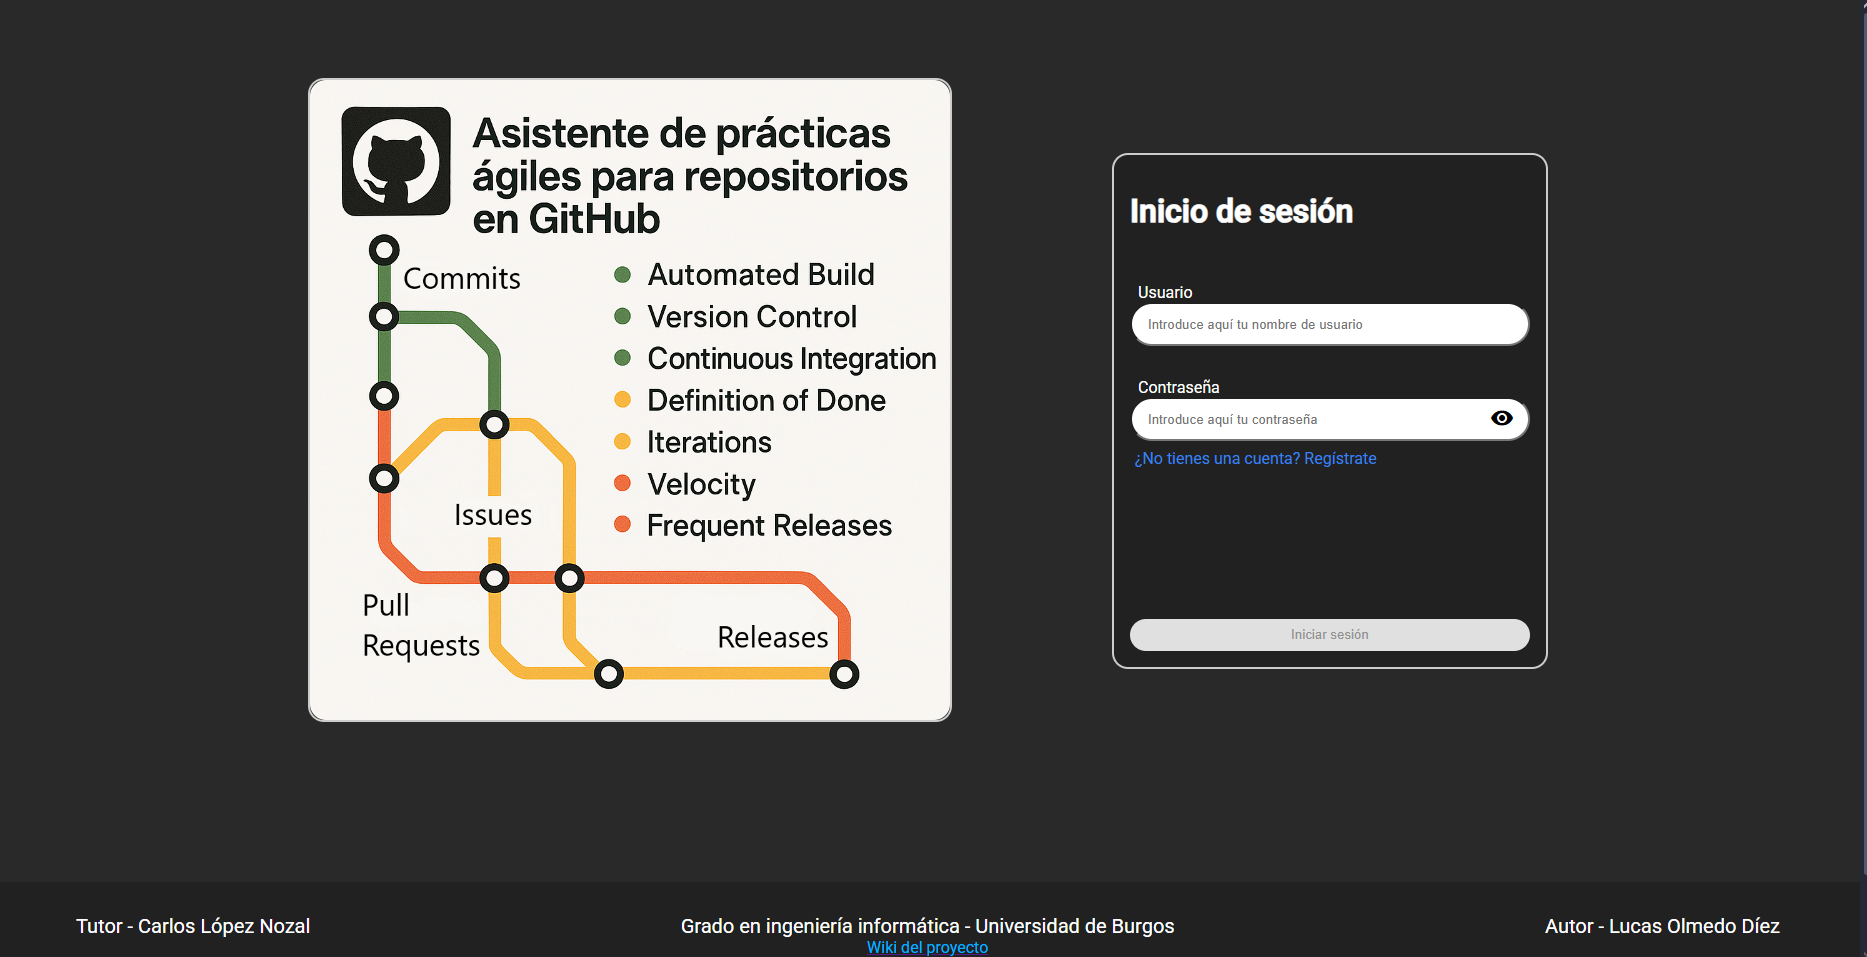
\includegraphics[width=0.8\textwidth]{img/E1-login.png}
\caption{E1: Inicio de sesión del usuario}
\label{fig:E1-login}
\end{figure}

\begin{figure}[H]
\centering
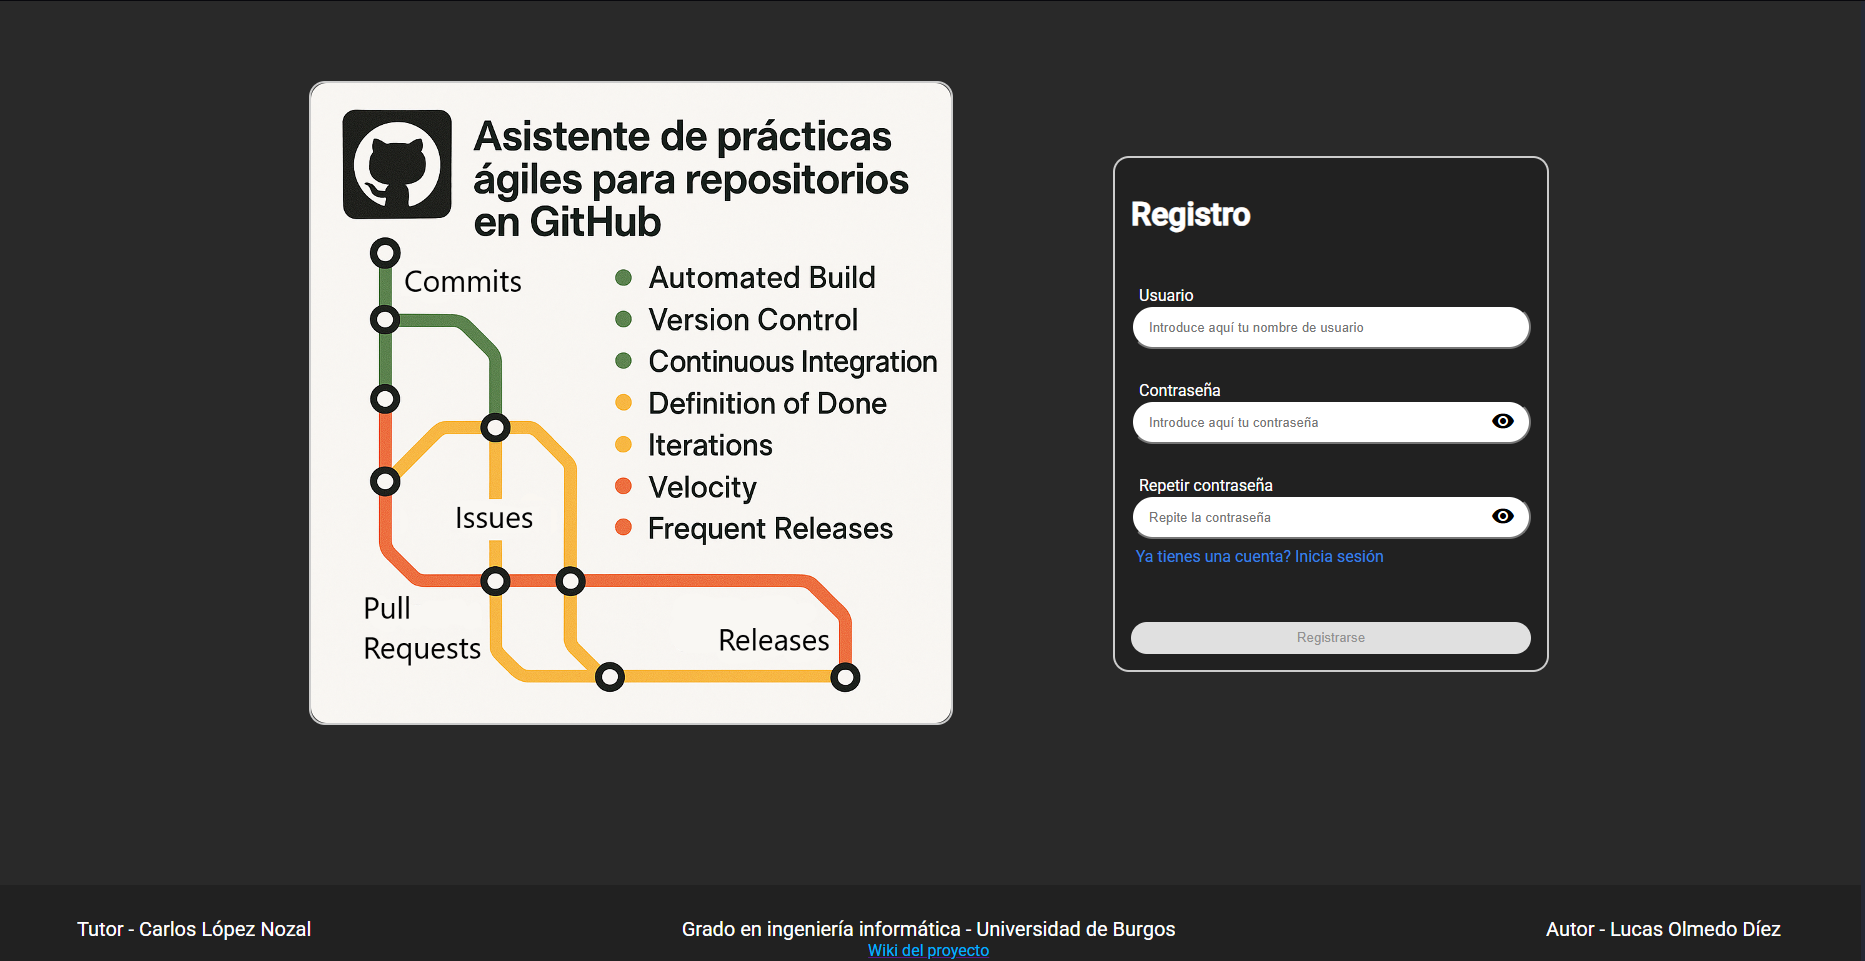
\includegraphics[width=0.8\textwidth]{img/E2-register.png}
\caption{E2: registro del usuario}
\label{fig:E2-register}
\end{figure}

\begin{itemize}
    \item El usuario accede a la página de registro o inicio de sesión.
    \item El usuario introduce los datos necesarios (usuario y contraseña).
    \item El sistema verifica la validez de los datos.
    \item El sistema registra al usuario o permite el acceso según corresponda.
\end{itemize}

\newpage
\subsection{Configuración de la cuenta}

Permite al usuario cambiar la contraseña y modificar el idioma de la aplicación.

\begin{figure}[H]
\centering

\includegraphics[width=0.8\textwidth]{img/E3-user-configuration.png}
\caption{E3: configuración del usuario}
\label{fig:E3-user-configuration}
\end{figure}

\begin{itemize}
    \item El usuario puede cambiar el idioma de la interfaz entre inglés y español mediante el icono de la bandera
    \item El usuario pulsa la opción de cambio de contraseña e introduce los datos necesarios (usuario, contraseña actual y nueva contraseña).
    \item El sistema verifica la validez de los datos.
    \item El sistema cambia la contraseña del usuario e inicia sesión automáticamente.
\end{itemize}

\newpage
\subsection{Introducción y validación de URLs de repositorios}

Permite al usuario introducir URLs de repositorios GitHub y valida su formato y accesibilidad.

\begin{figure}[H]
\centering
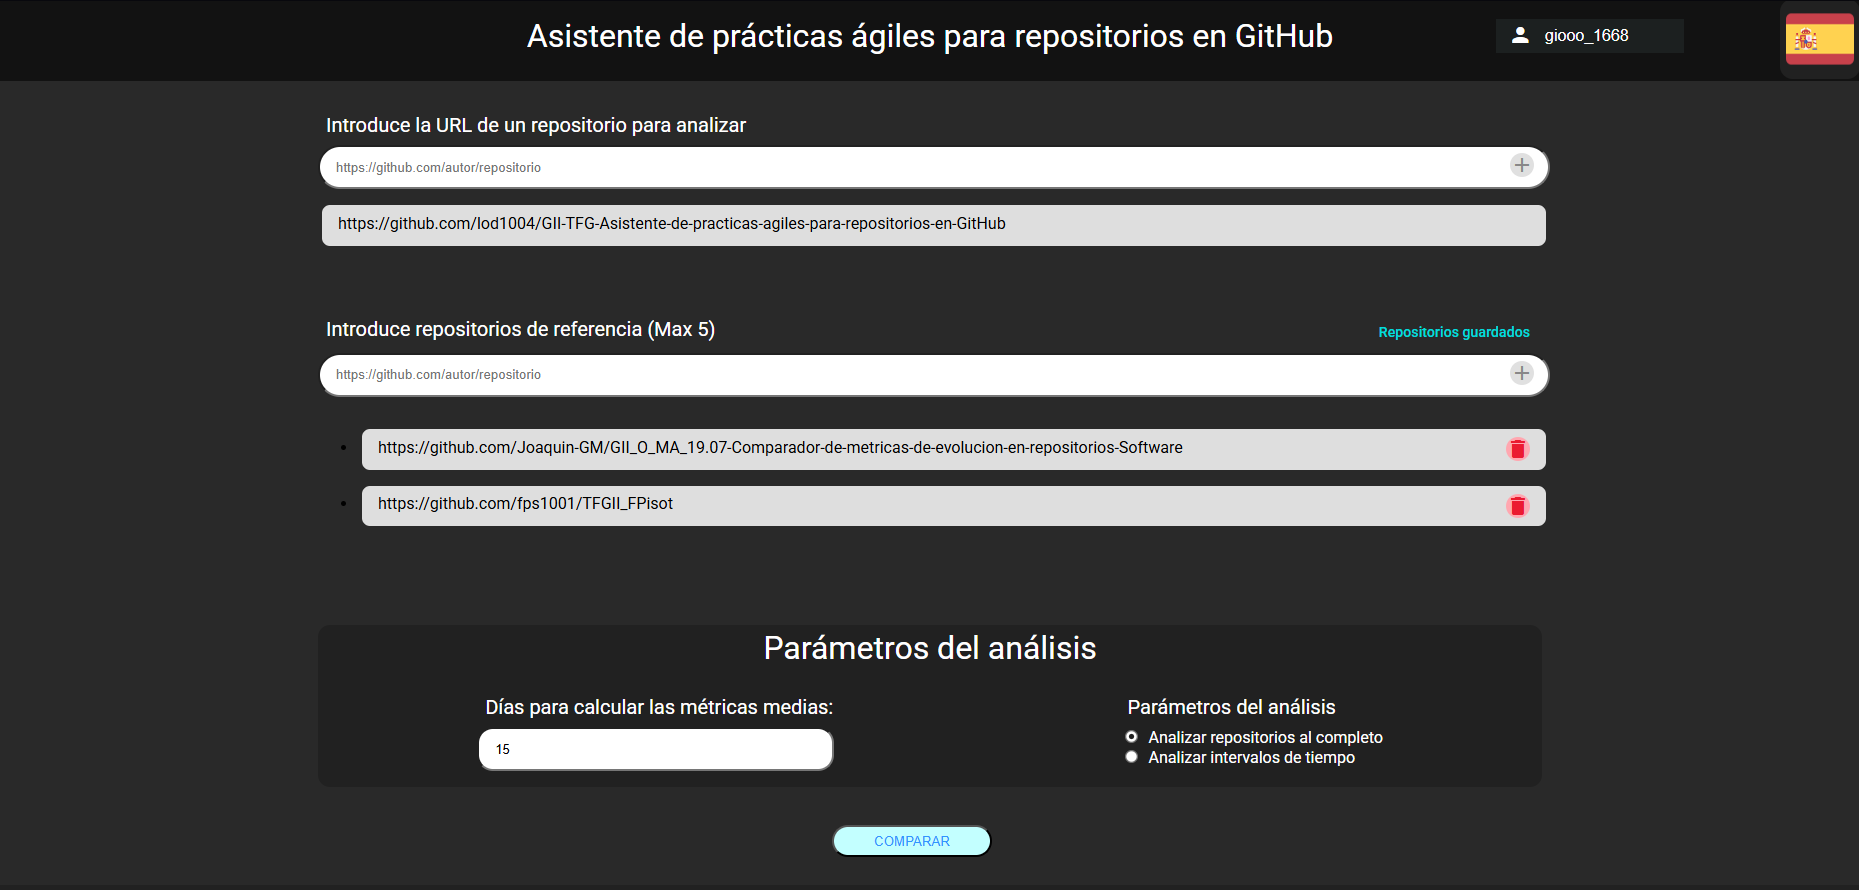
\includegraphics[width=0.8\textwidth]{img/E4-urls.png}
\caption{E4: Validación de URLs de repositorios}
\label{fig:E4-urls}
\end{figure}

\begin{itemize}
    \item El usuario introduce una URL de repositorio a analizar y una o varias URLs de repositorios de referencia.
    \item El sistema valida las urls.
\end{itemize}

\newpage
\subsection{Configurar análisis del repositorio}

El usuario configura cómo se analizarán los datos del repositorio: número de días para calcular las métricas temporales, análisis completo o por intervalos intervalos absolutos o relativos períodos de los intervalos.

\begin{figure}[H]
\centering
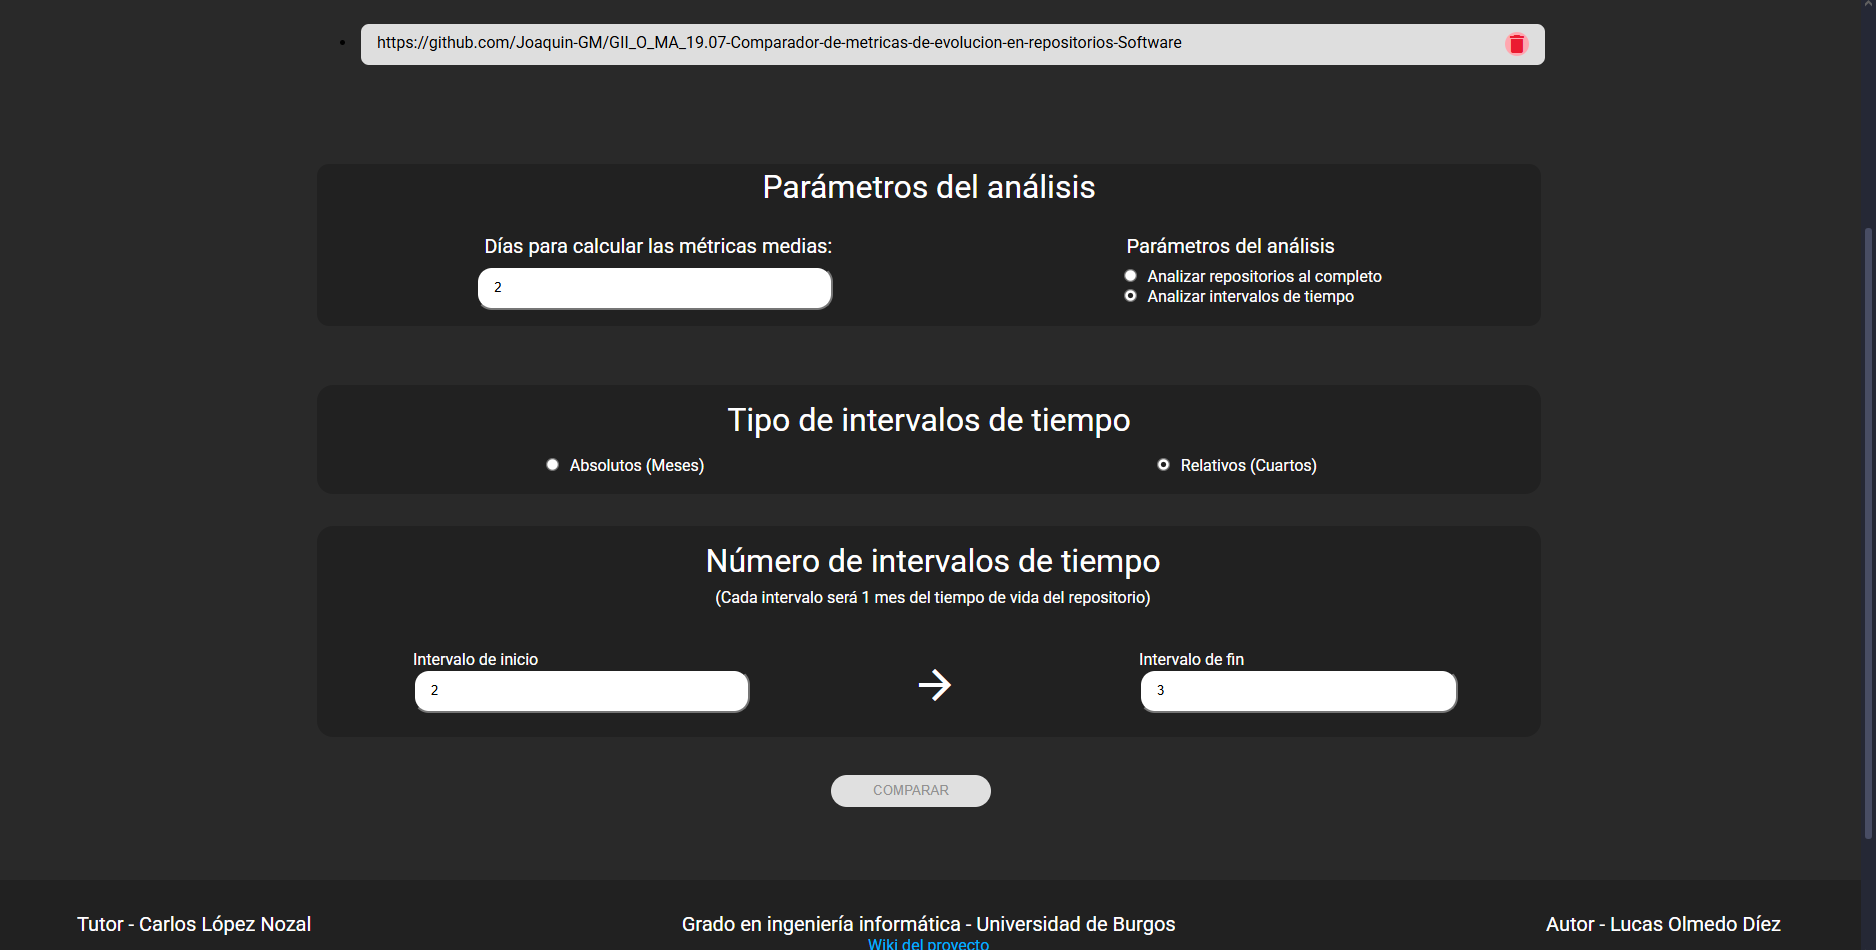
\includegraphics[width=0.8\textwidth]{img/E4.1-configuracion-analisis.png}
\caption{E4.1: Configuración del análisis de los repositorios}
\label{fig:E4.1-configuracion-analisis}
\end{figure}

\begin{itemize}
    \item El usuario selecciona si analizar los repositorios al completo por intervalos.
    \item Ajusta el número de días para calcular las métricas de medias.
    \item Elige el tipo de intervalos etre absolutos o relativos.
    \item Se eligen los intervalos del análisis.
\end{itemize}

\newpage
\subsection{Gestionar grupos de repositorios de comparación}

Permite al usuario cargar o borrar grupos de repositorios previamente guardados para usarlos como referencia comparativa en los análisis.

\begin{figure}[H]
\centering
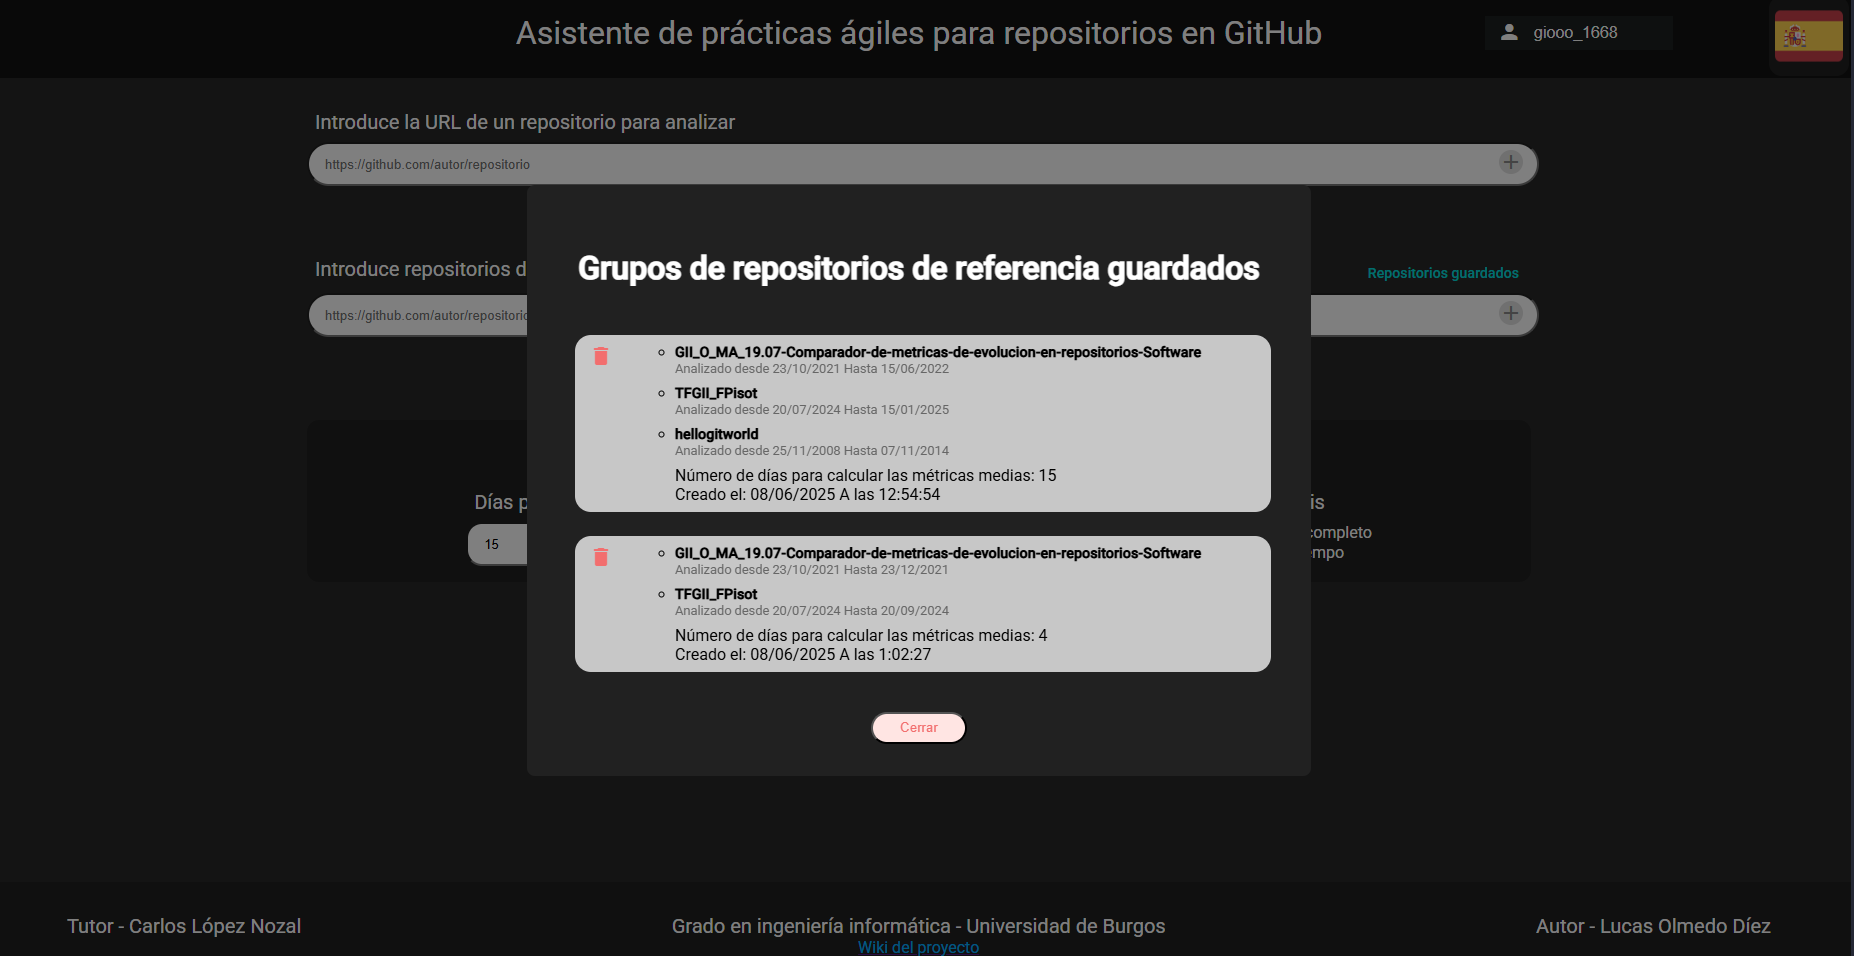
\includegraphics[width=0.8\textwidth]{img/E5-grupos.png}
\caption{E5: Gestión de grupos de repositorios}
\label{fig:E5-grupos}
\end{figure}

\begin{itemize}
    \item El usuario accede a la sección de gestión de repositorios guardados.
    \item Selecciona un grupo de repositorios guardado previamente y lo carga.
    \item (Opcional) Elimina uno o más grupos guardados si lo desea.
\end{itemize}

\newpage
\subsection{Visualizar evaluación de buenas prácticas ágiles}

Permite al usuario visualizar el grado de adopción de buenas prácticas ágiles evaluadas automáticamente por el sistema a partir de los datos del repositorio.

\begin{figure}[H]
\centering
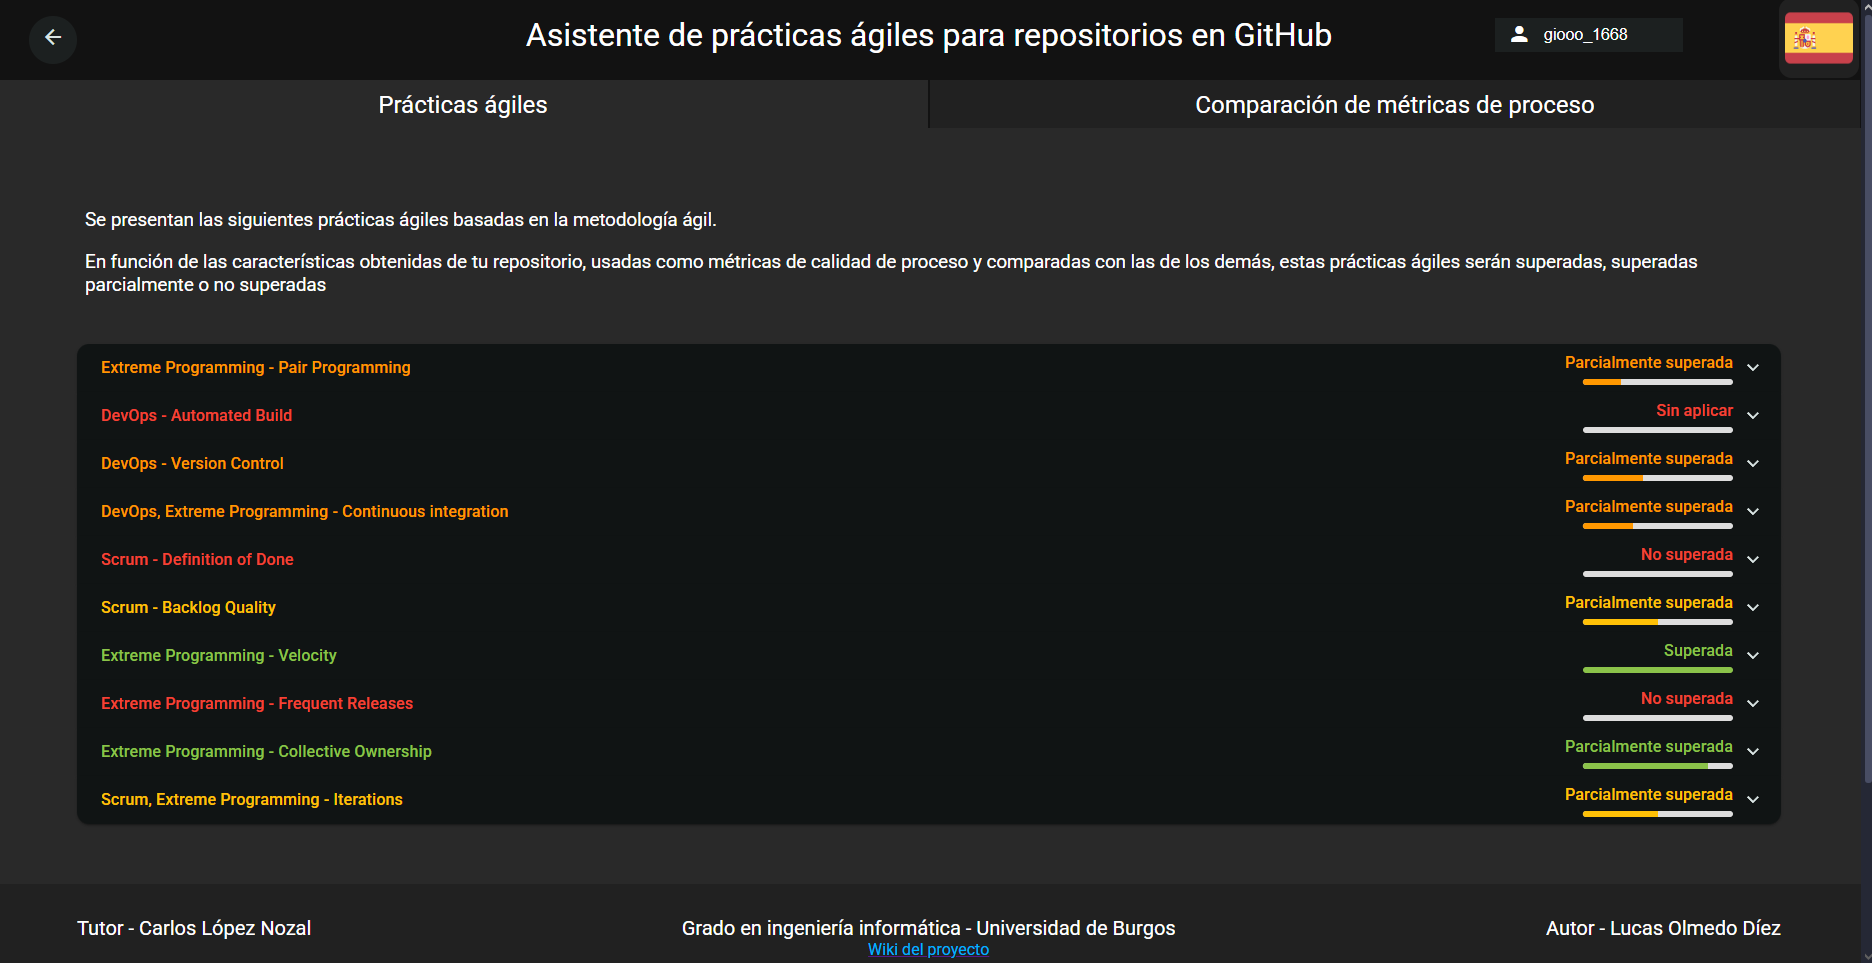
\includegraphics[width=0.8\textwidth]{img/E6-practicas-agiles.png}
\caption{E6: Evaluación de buenas prácticas ágiles}
\label{fig:E6-practicas-agiles}
\end{figure}

\begin{figure}[H]
\centering
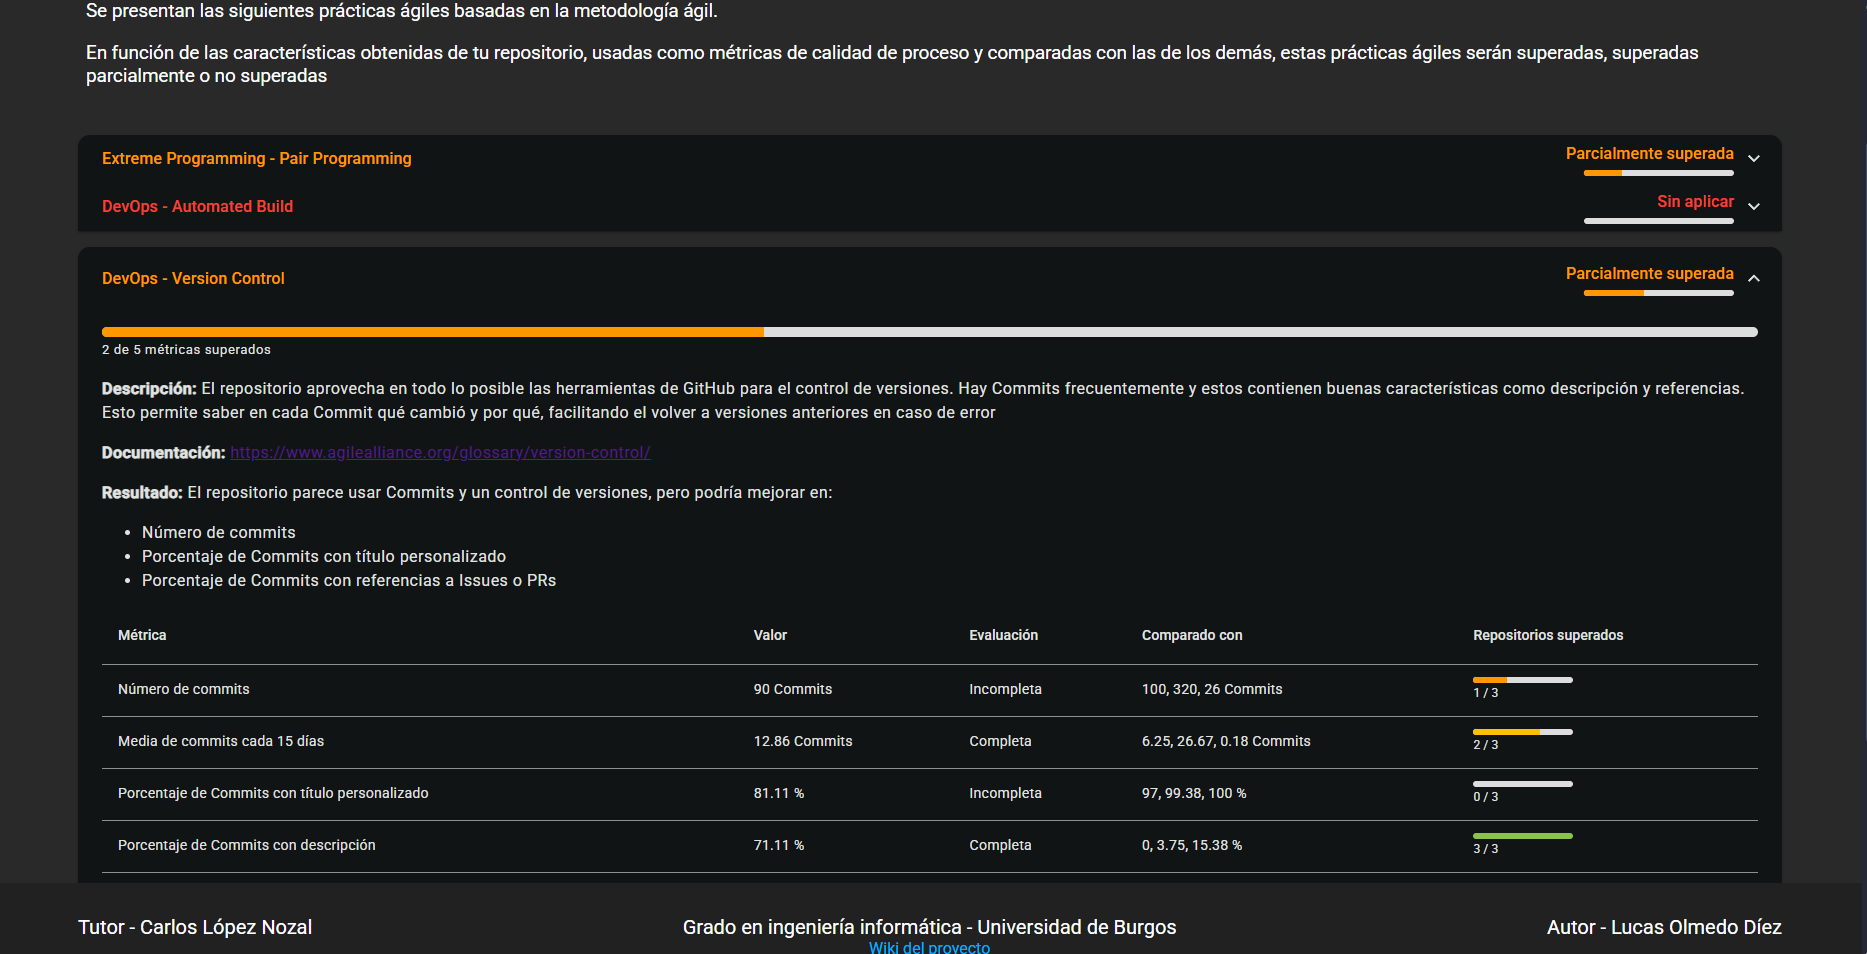
\includegraphics[width=0.8\textwidth]{img/E6.1-detalle-practicas-agiles.png}
\caption{E6: Detalle de las prácticas ágiles}
\label{fig:E6.1-detalle-practicas-agiles}
\end{figure}

\begin{itemize}
    \item El sistema muestra los resultados del análisis de buenas prácticas en formato gráfico y textual.
    \item El usuario puede seleccionar cada práctica ágil para ver los detalles de su evaluación y comparación entre repositorios.
\end{itemize}

\newpage
\subsection{ Comparar medidas de calidad de proceso con repositorios de referencia}

Permite comparar visualmente las métricas del repositorio analizado con las de los repositorios de referencia cargados.

\begin{figure}[H]
\centering
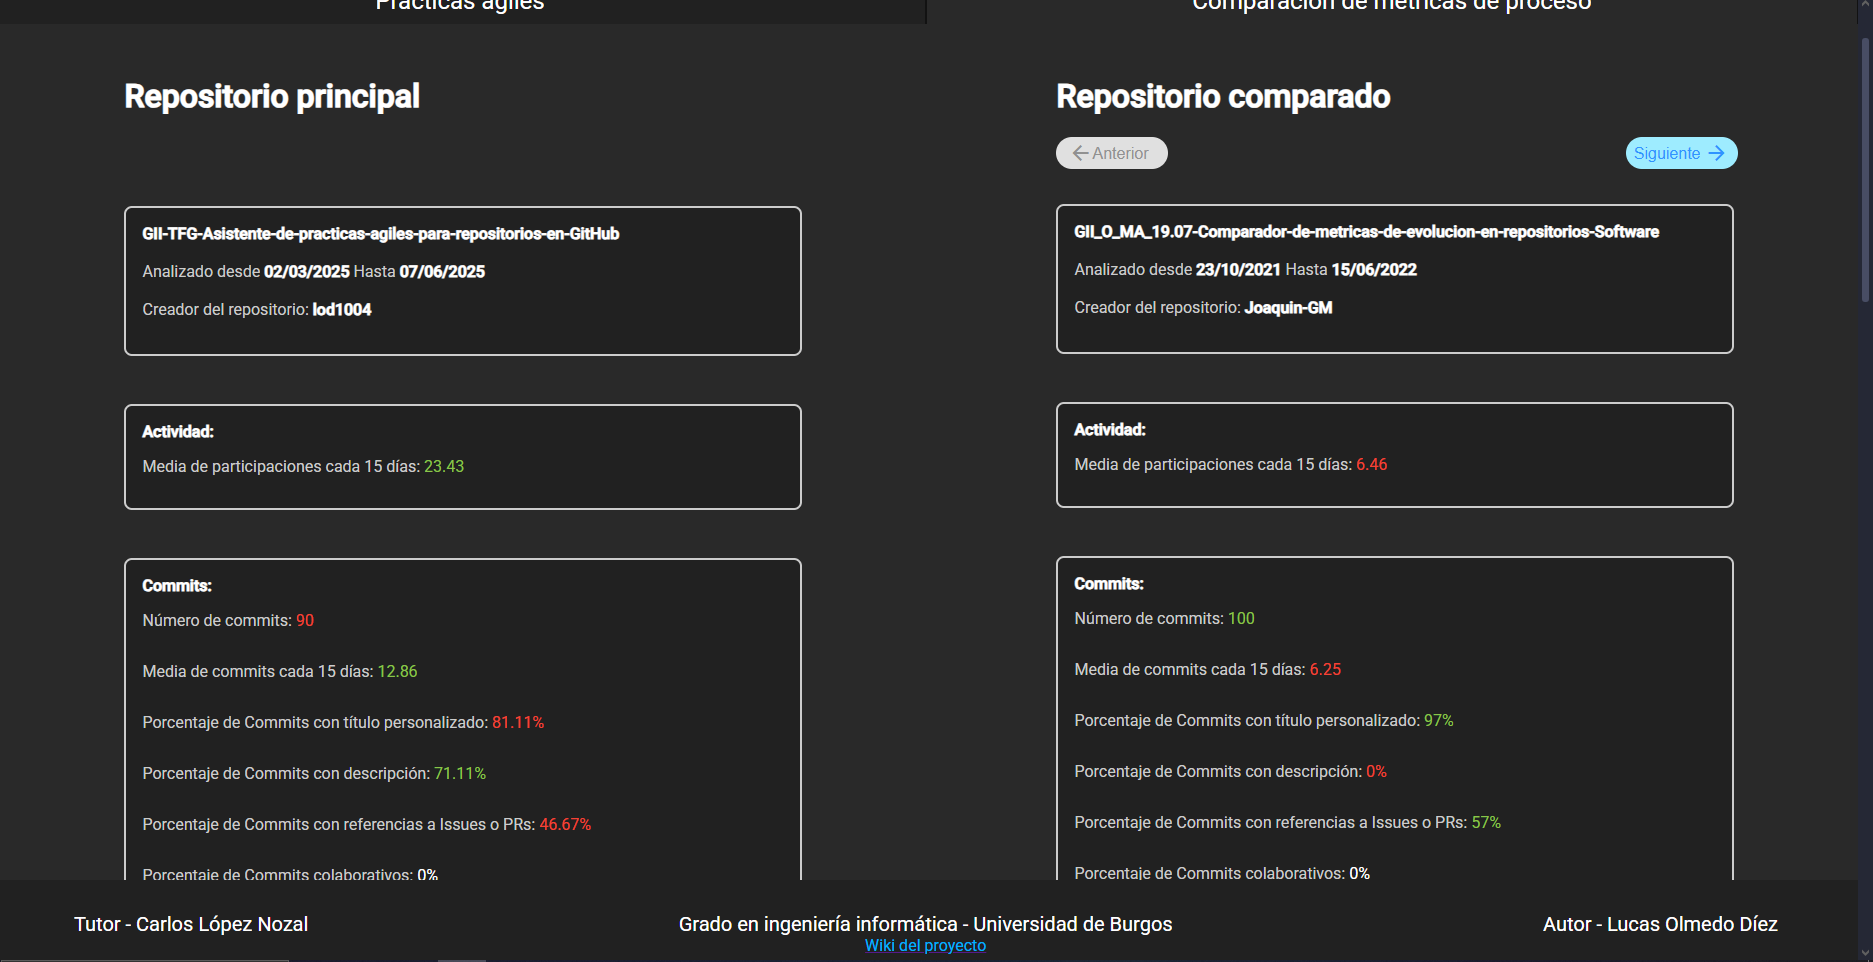
\includegraphics[width=0.8\textwidth]{img/E7-metricas.png}
\caption{E7: Comparación con repositorios de referencia}
\label{fig:E7-metricas}
\end{figure}

\begin{itemize}
    \item El usuario accede a la sección de comparación.
    \item El sistema genera y muestra listas comparativas de las métricas seleccionadas.
    \item El usuario puede elegir qué repositorio de referencia mostrar para compararlo.
\end{itemize}
